The matplotlib basemap toolkit is an add-on for matplotlib that provides
the capability to draw maps of the earth in various map projections,
and plot data on those maps. This section shows how to use basemap
to create simple maps, draw coastlines and political boundaries, draw
lines of constant latitude and longitude, and plot geophysical data
on the maps.


\section{Setting up the map.}

In order to represent the curved surface of the earth in a two-dimensional
map, a map projection is needed. Since this cannot be done without
distortion, there are many map projections, each with it's own advantages
and disadvantages. Basemap provides 19 different map projections.
Some are global, some can only represent a portion of the globe. When
a Basemap class instance is created, the desired map projection must
be specified, along with information about the portion of the earth's
surface that the map projection will describe. There are two basic
ways of doing this. One is to provide the latitude and longitude values
of each of the four corners of the rectangular map projection region.
The other is to provide the lat/lon value of the center of the map
projection region along with the width and height of the region in
map projection coordinates. The first script illustrates how to use
both of these methods to create a simple map. It also shows how to
draw the continents and political boundaries on the map.

Here is an example script that creates a map by specifying the latitudes
and longitudes of the four corners

\lstinputlisting[label=code:basemap1_skel,caption={IGNORED}]{../examples/basemap1.py}

After running this script, you should see a plot that looks similar
to Figure 1.

\begin{figure}[h]
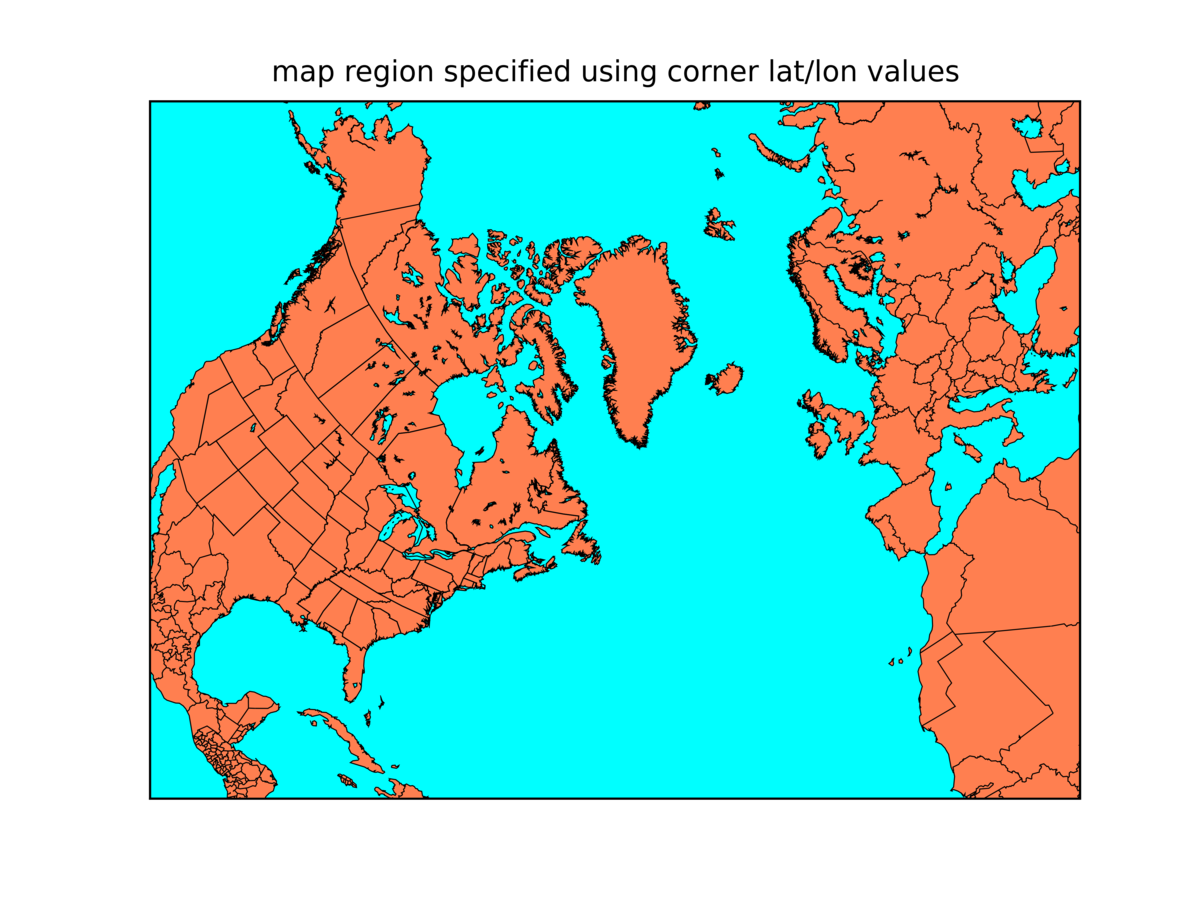
\includegraphics[scale=0.75]{fig/basemap1}

\caption{A map created by specifying the latitudes and longitudes of the four
corners.}

\end{figure}

\medskip{}
Here is an example script that creates a map by specifying the center
of the map, plus the width and height in meters.

\lstinputlisting[label=code:basemap2_skel,caption={IGNORED}]{../examples/basemap2.py}

After running this script, you should see a plot that looks nearly
identical to Figure 1.\medskip{}


The Basemap class instance can be used to convert latitudes and longitudes
to coordinates on the map. To do this, simply call the instance as
if it were a function, passing it the longitude and latitudes values
to convert. The corresponding x and y values in map projection coordinates
will be returned. The following example script shows how to use this
to plot the locations of two cities (New York and London). The Basemap
method drawgreatcircle is then used to draw the great circle route
between these cities on the map.

\lstinputlisting[label=code:basemap3_skel,caption={IGNORED}]{../examples/basemap3.py}

This should produce something similar to Figure 2.

\begin{figure}[h]
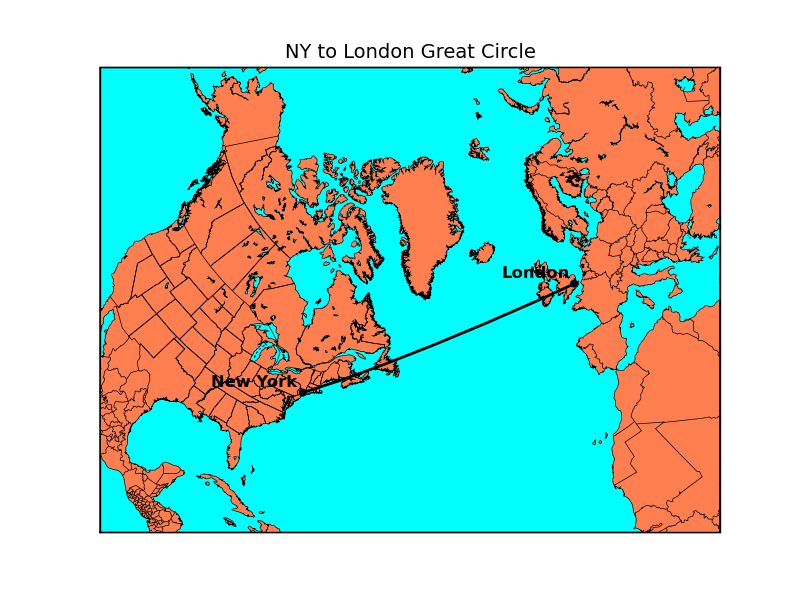
\includegraphics[scale=0.75]{fig/basemap3}

\caption{Drawing the locations of two cities, and connecting them along a great
circle.}

\end{figure}

\medskip{}
Most maps include a graticule grid, a reference network of labelled
latitude and longitude lines. Basemap does this with the drawparallels
and drawmeridians instance methods. The longitude and latitude lines
can be labelled where the intersect the map projection boundary. Following
is an example script that draws a graticule on the map we've been
working with.

\lstinputlisting[label=code:basemap4_skel,caption={IGNORED}]{../examples/basemap4.py}

Running this script should produce a plot that looks like Figure 3.

\begin{figure}[h]
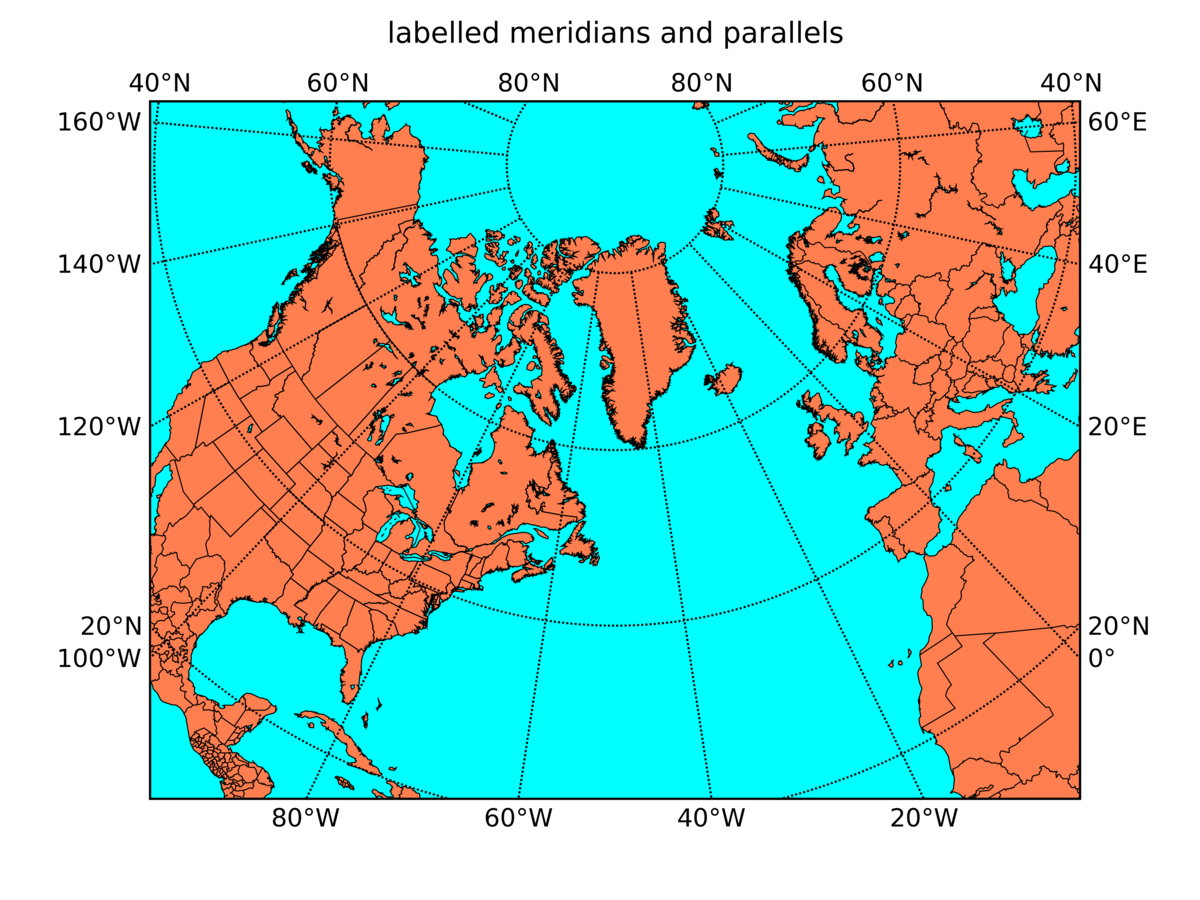
\includegraphics[scale=0.75]{fig/basemap4}

\caption{Drawing labelled meridians and parallels on the map (a graticule grid).}

\end{figure}


\section{Plotting geophysical data on the map.}

One of the most common uses of Basemap is to visualize earth science
data, such as output from climate models. These data often come on
latitude/longitude grids. One common data format for storing such
grids is NetCDF. Basemap includes a NetCDF file reader (written in
pure python by Roberto D'Almeida). There are python packages available
for reading just about every other scientific data format imaginable,
including HDF, GRIB, FITS and many others. Following is an example
of how to read sea-surface temperature data from a NetCDF file and
plot it on a global mollweide projection.

\lstinputlisting[label=code:basemap5_skel,caption={IGNORED}]{../examples/basemap5.py}

The resulting plot should look like Figure 4.

\begin{figure}[h]
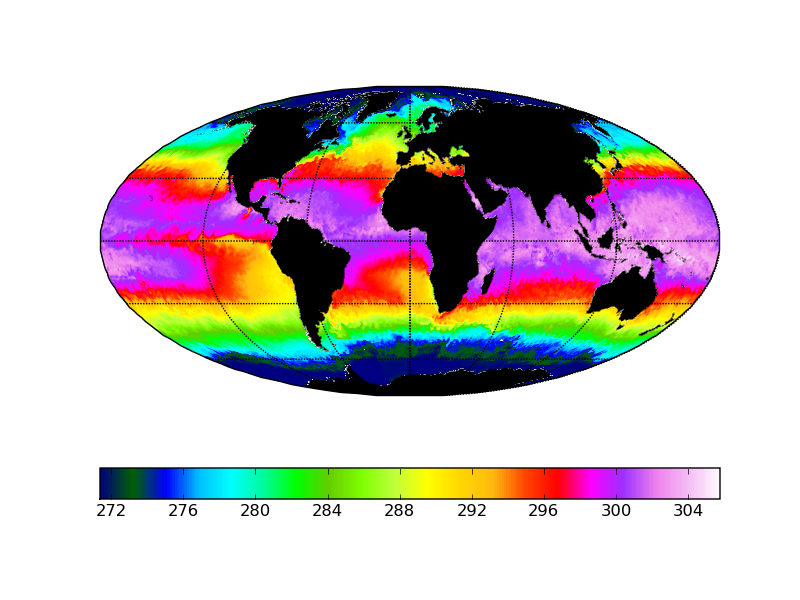
\includegraphics[scale=0.75]{fig/basemap5}

\caption{Sea surface temperature on a global mollweide projection.}

\end{figure}

\medskip{}

Basemap also is capable of reading ESRI shapefiles, a very common
GIS format. The script fillstates.py in the examples directory of
the basemap source distribution shows how to read and plot polygons
in a shapefile. There are many other useful examples in that directory
that illustrate various ways of using basemap.%
